\section{Appendix}\label{ap:appendix}
% PLOTS
\begin{figure}[H]
    \centering
    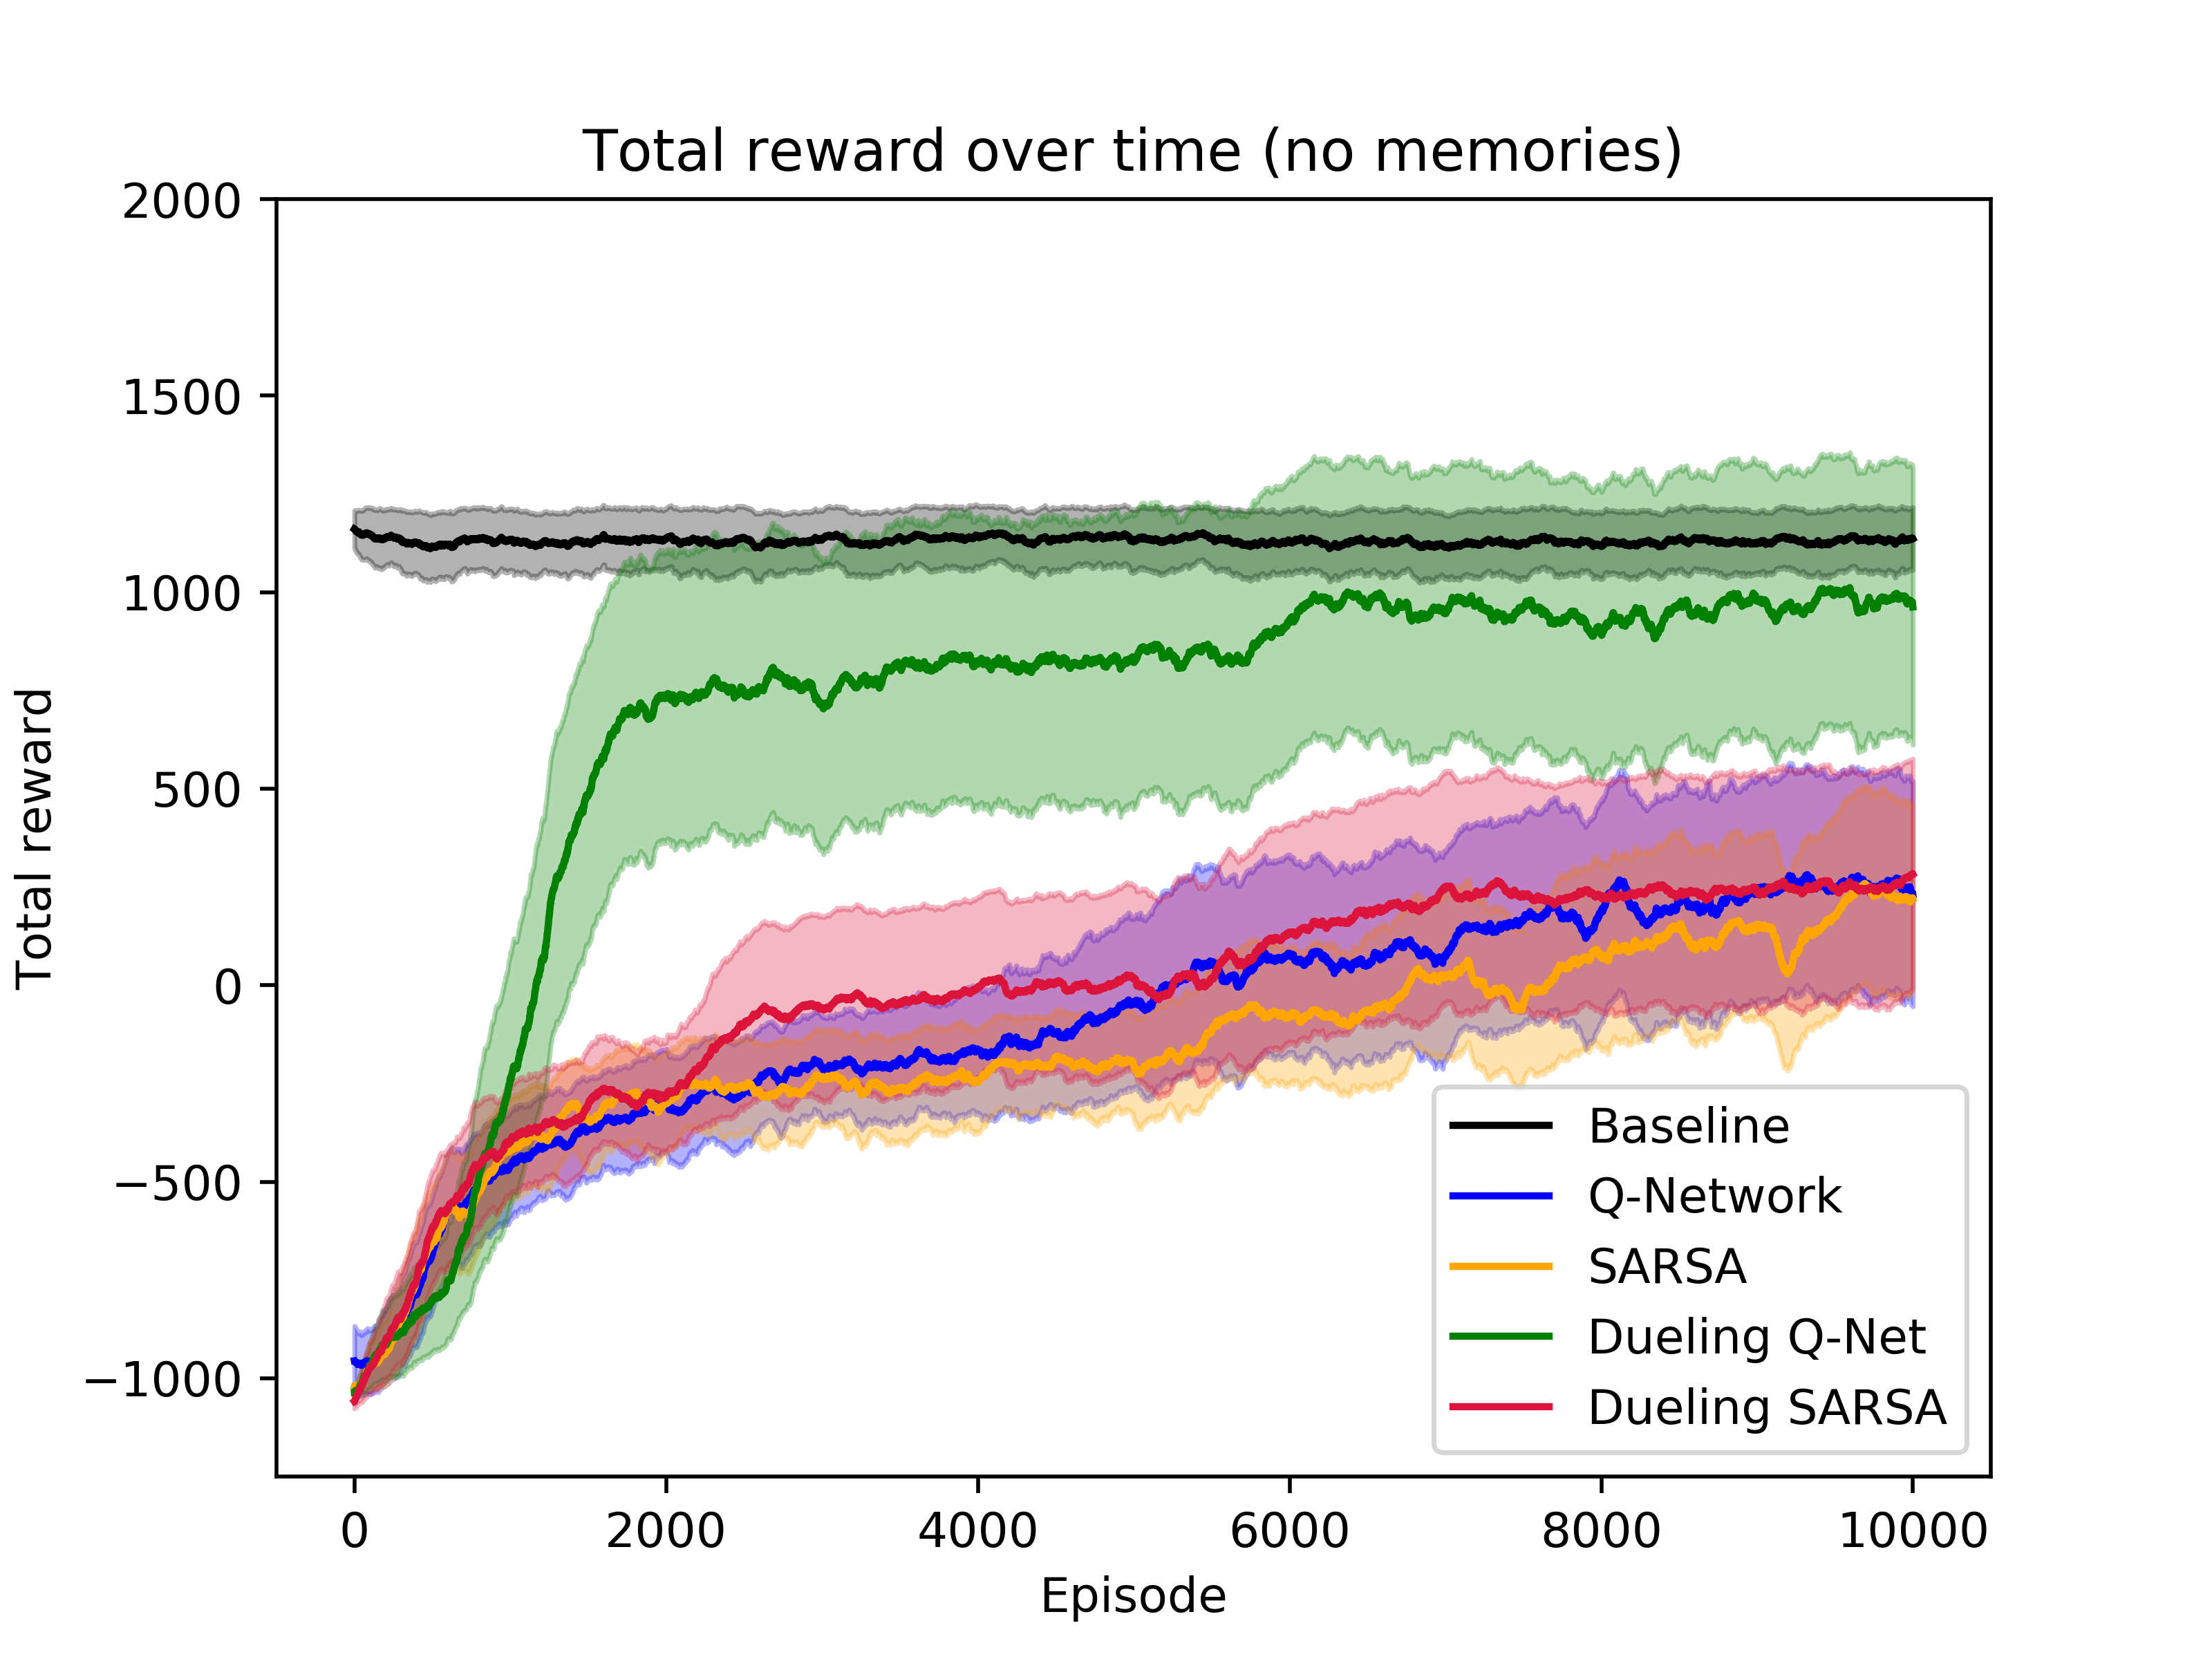
\includegraphics[width=\linewidth]{img/results/10-sized/total_rewards_0m-min.png}
    \caption{10-by-10 grid given no demonstation data.}
    \label{fig:10sized-nomem}
    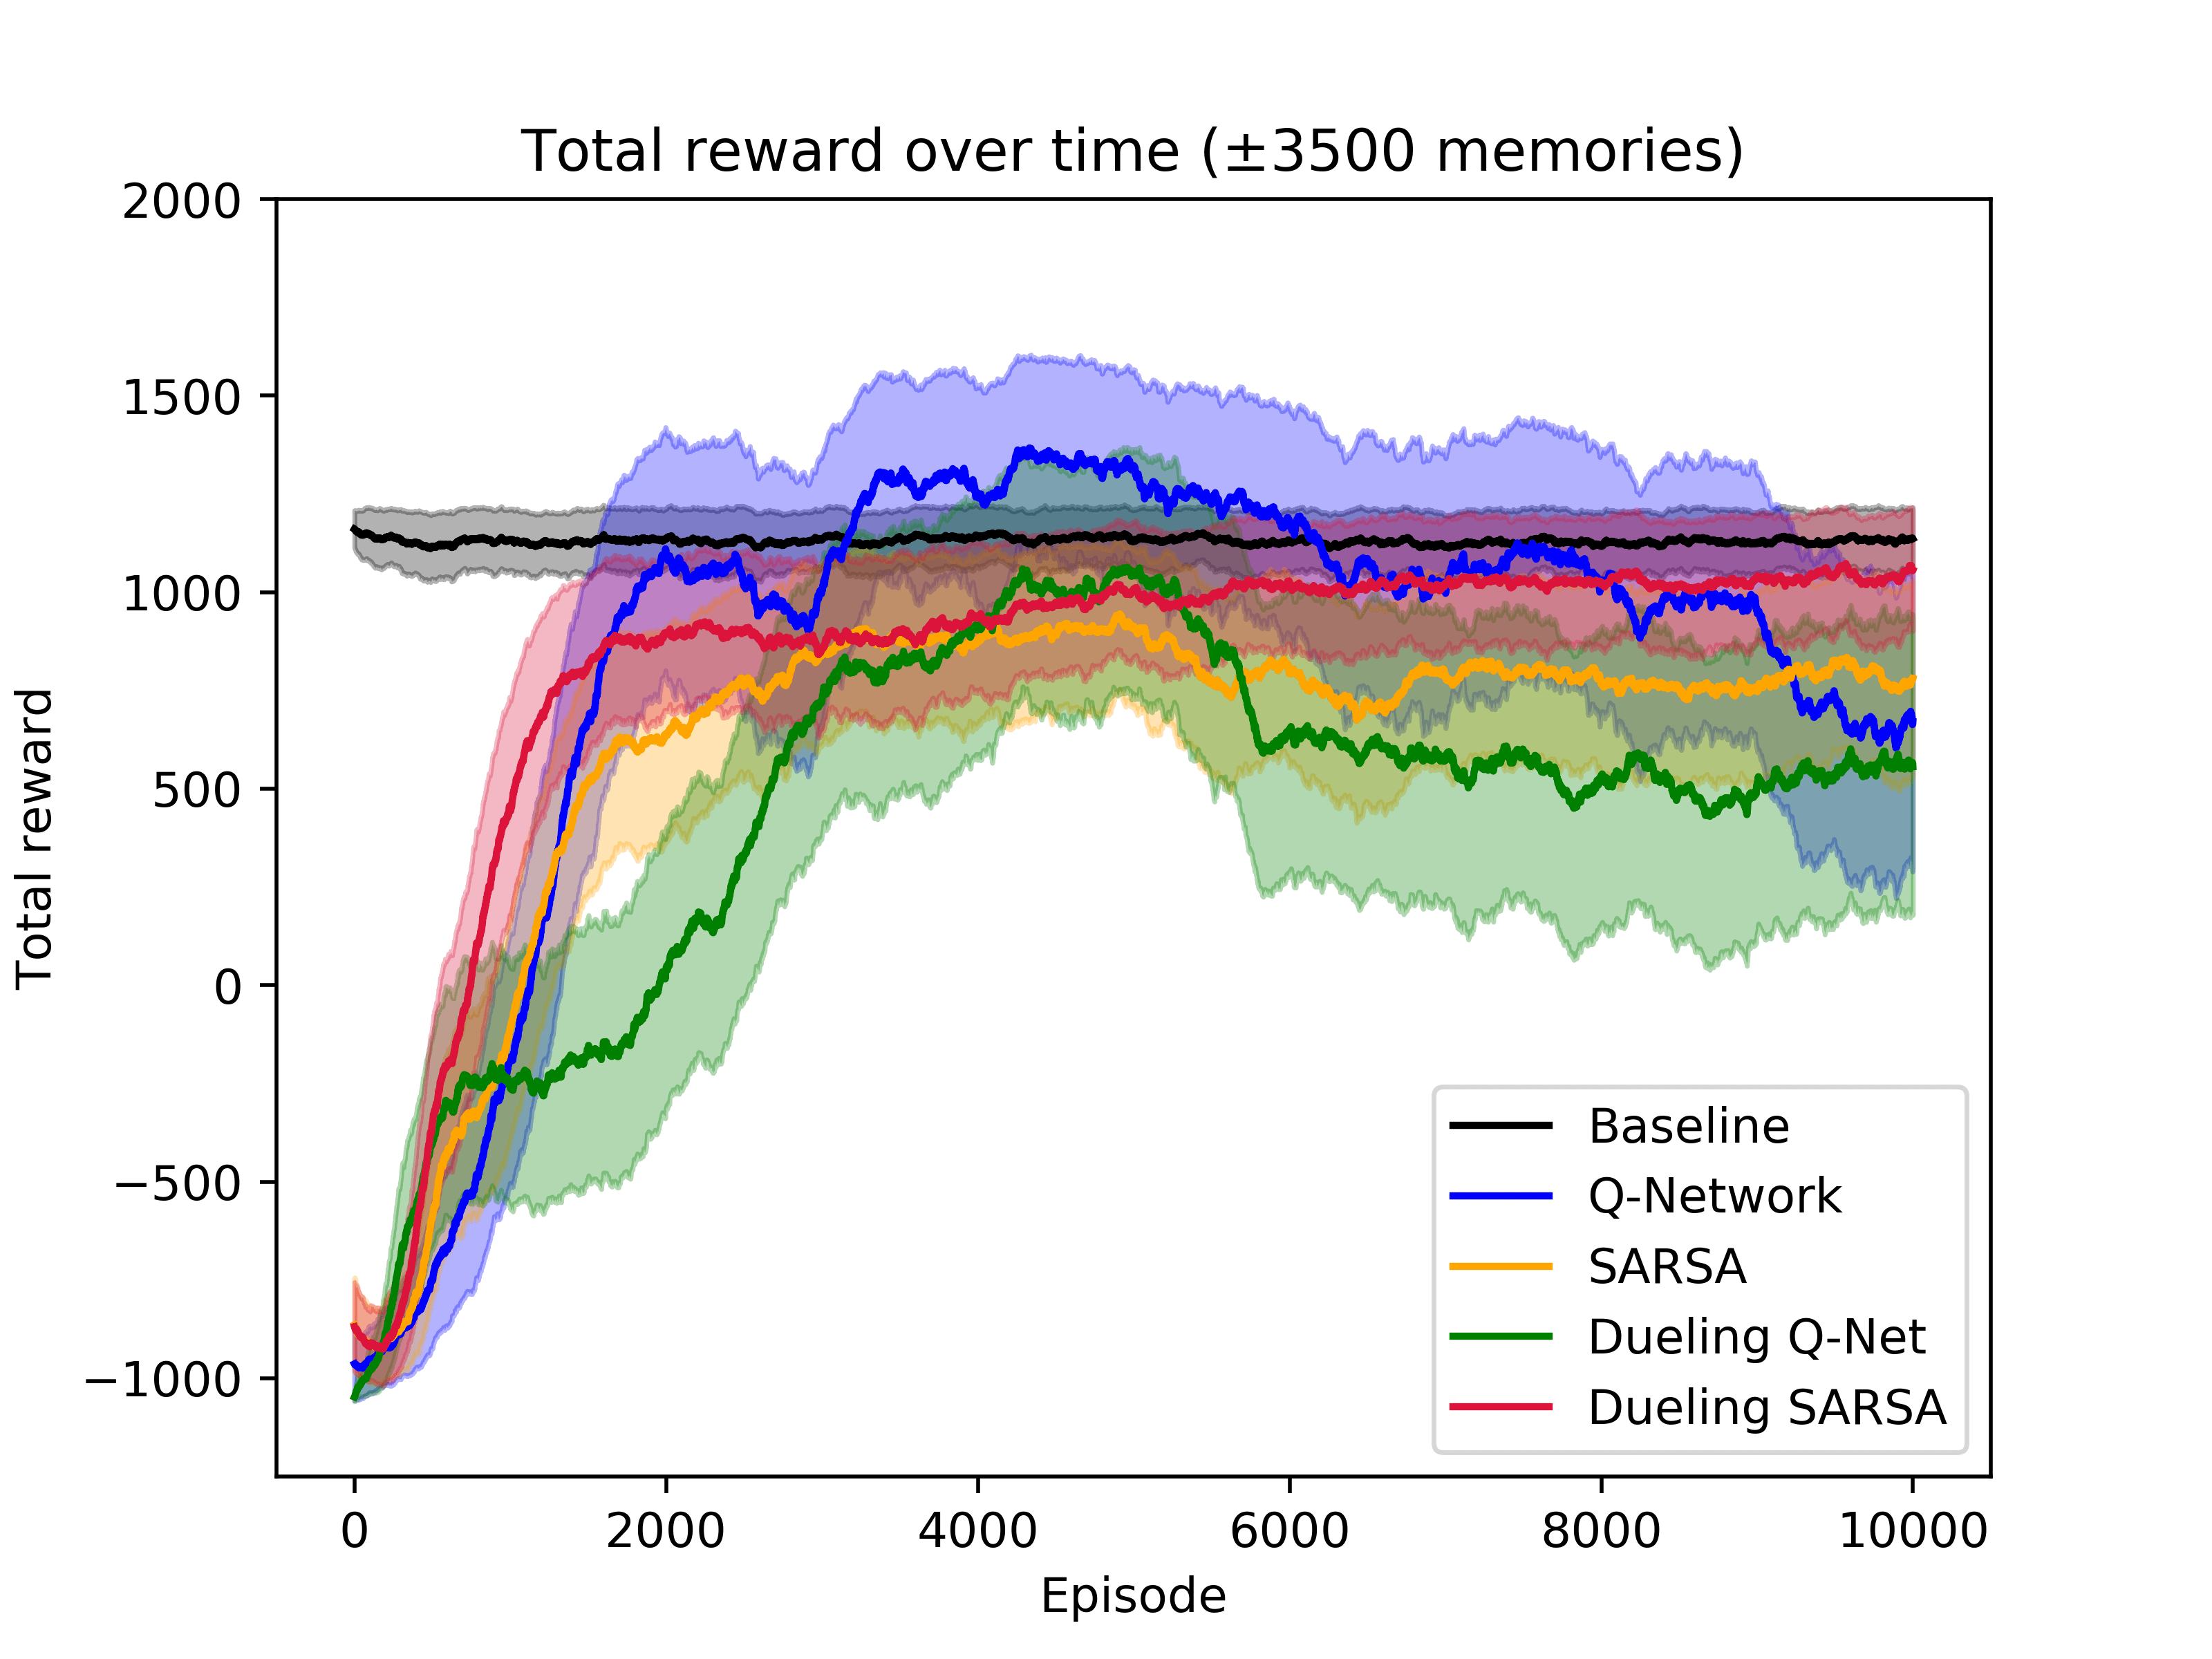
\includegraphics[width=\linewidth]{img/results/10-sized/total_rewards_100m-min.png}
    \caption{10-by-10 grid given 100 episodes of demonstation data.}
    \label{fig:10sized-100mem}
    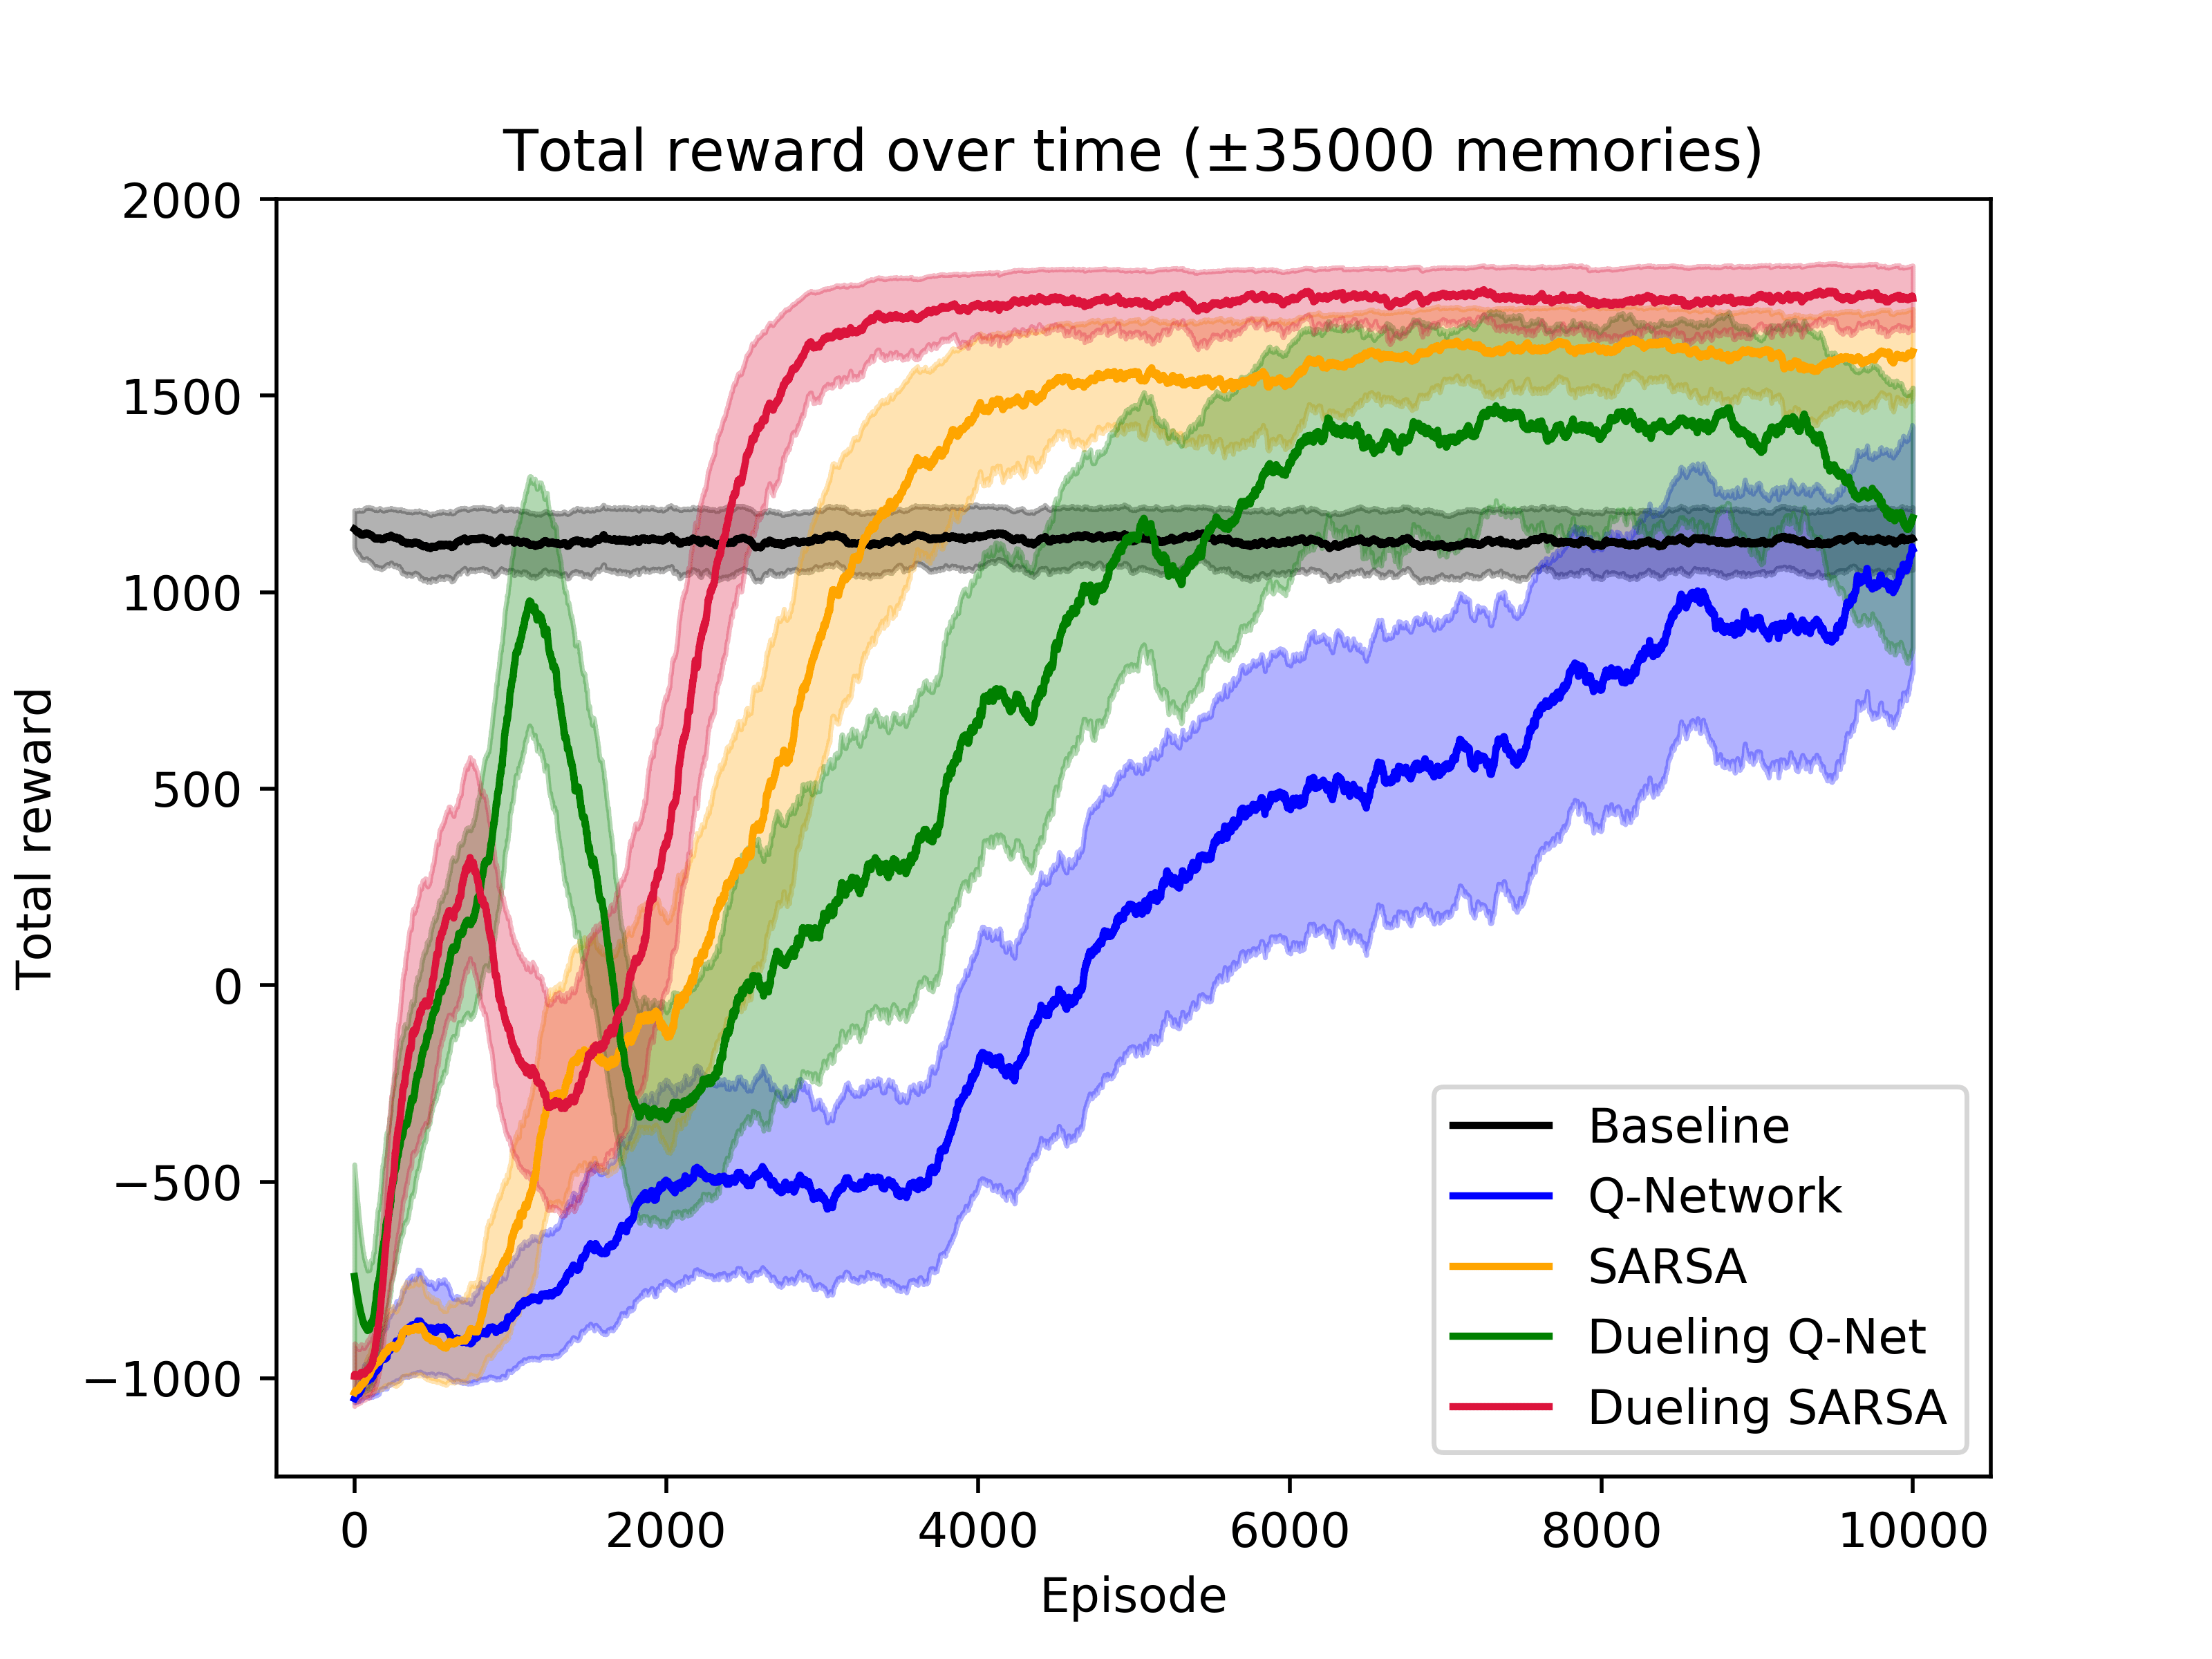
\includegraphics[width=\linewidth]{img/results/10-sized/total_rewards_1000m-min.png}
    \caption{10-by-10 grid given 1000 episodes of demonstation data.}
    \label{fig:10sized-1000mem}
\end{figure}
\hspace{1cm} %Fixes misalignment
\begin{figure}[H]
    \centering
    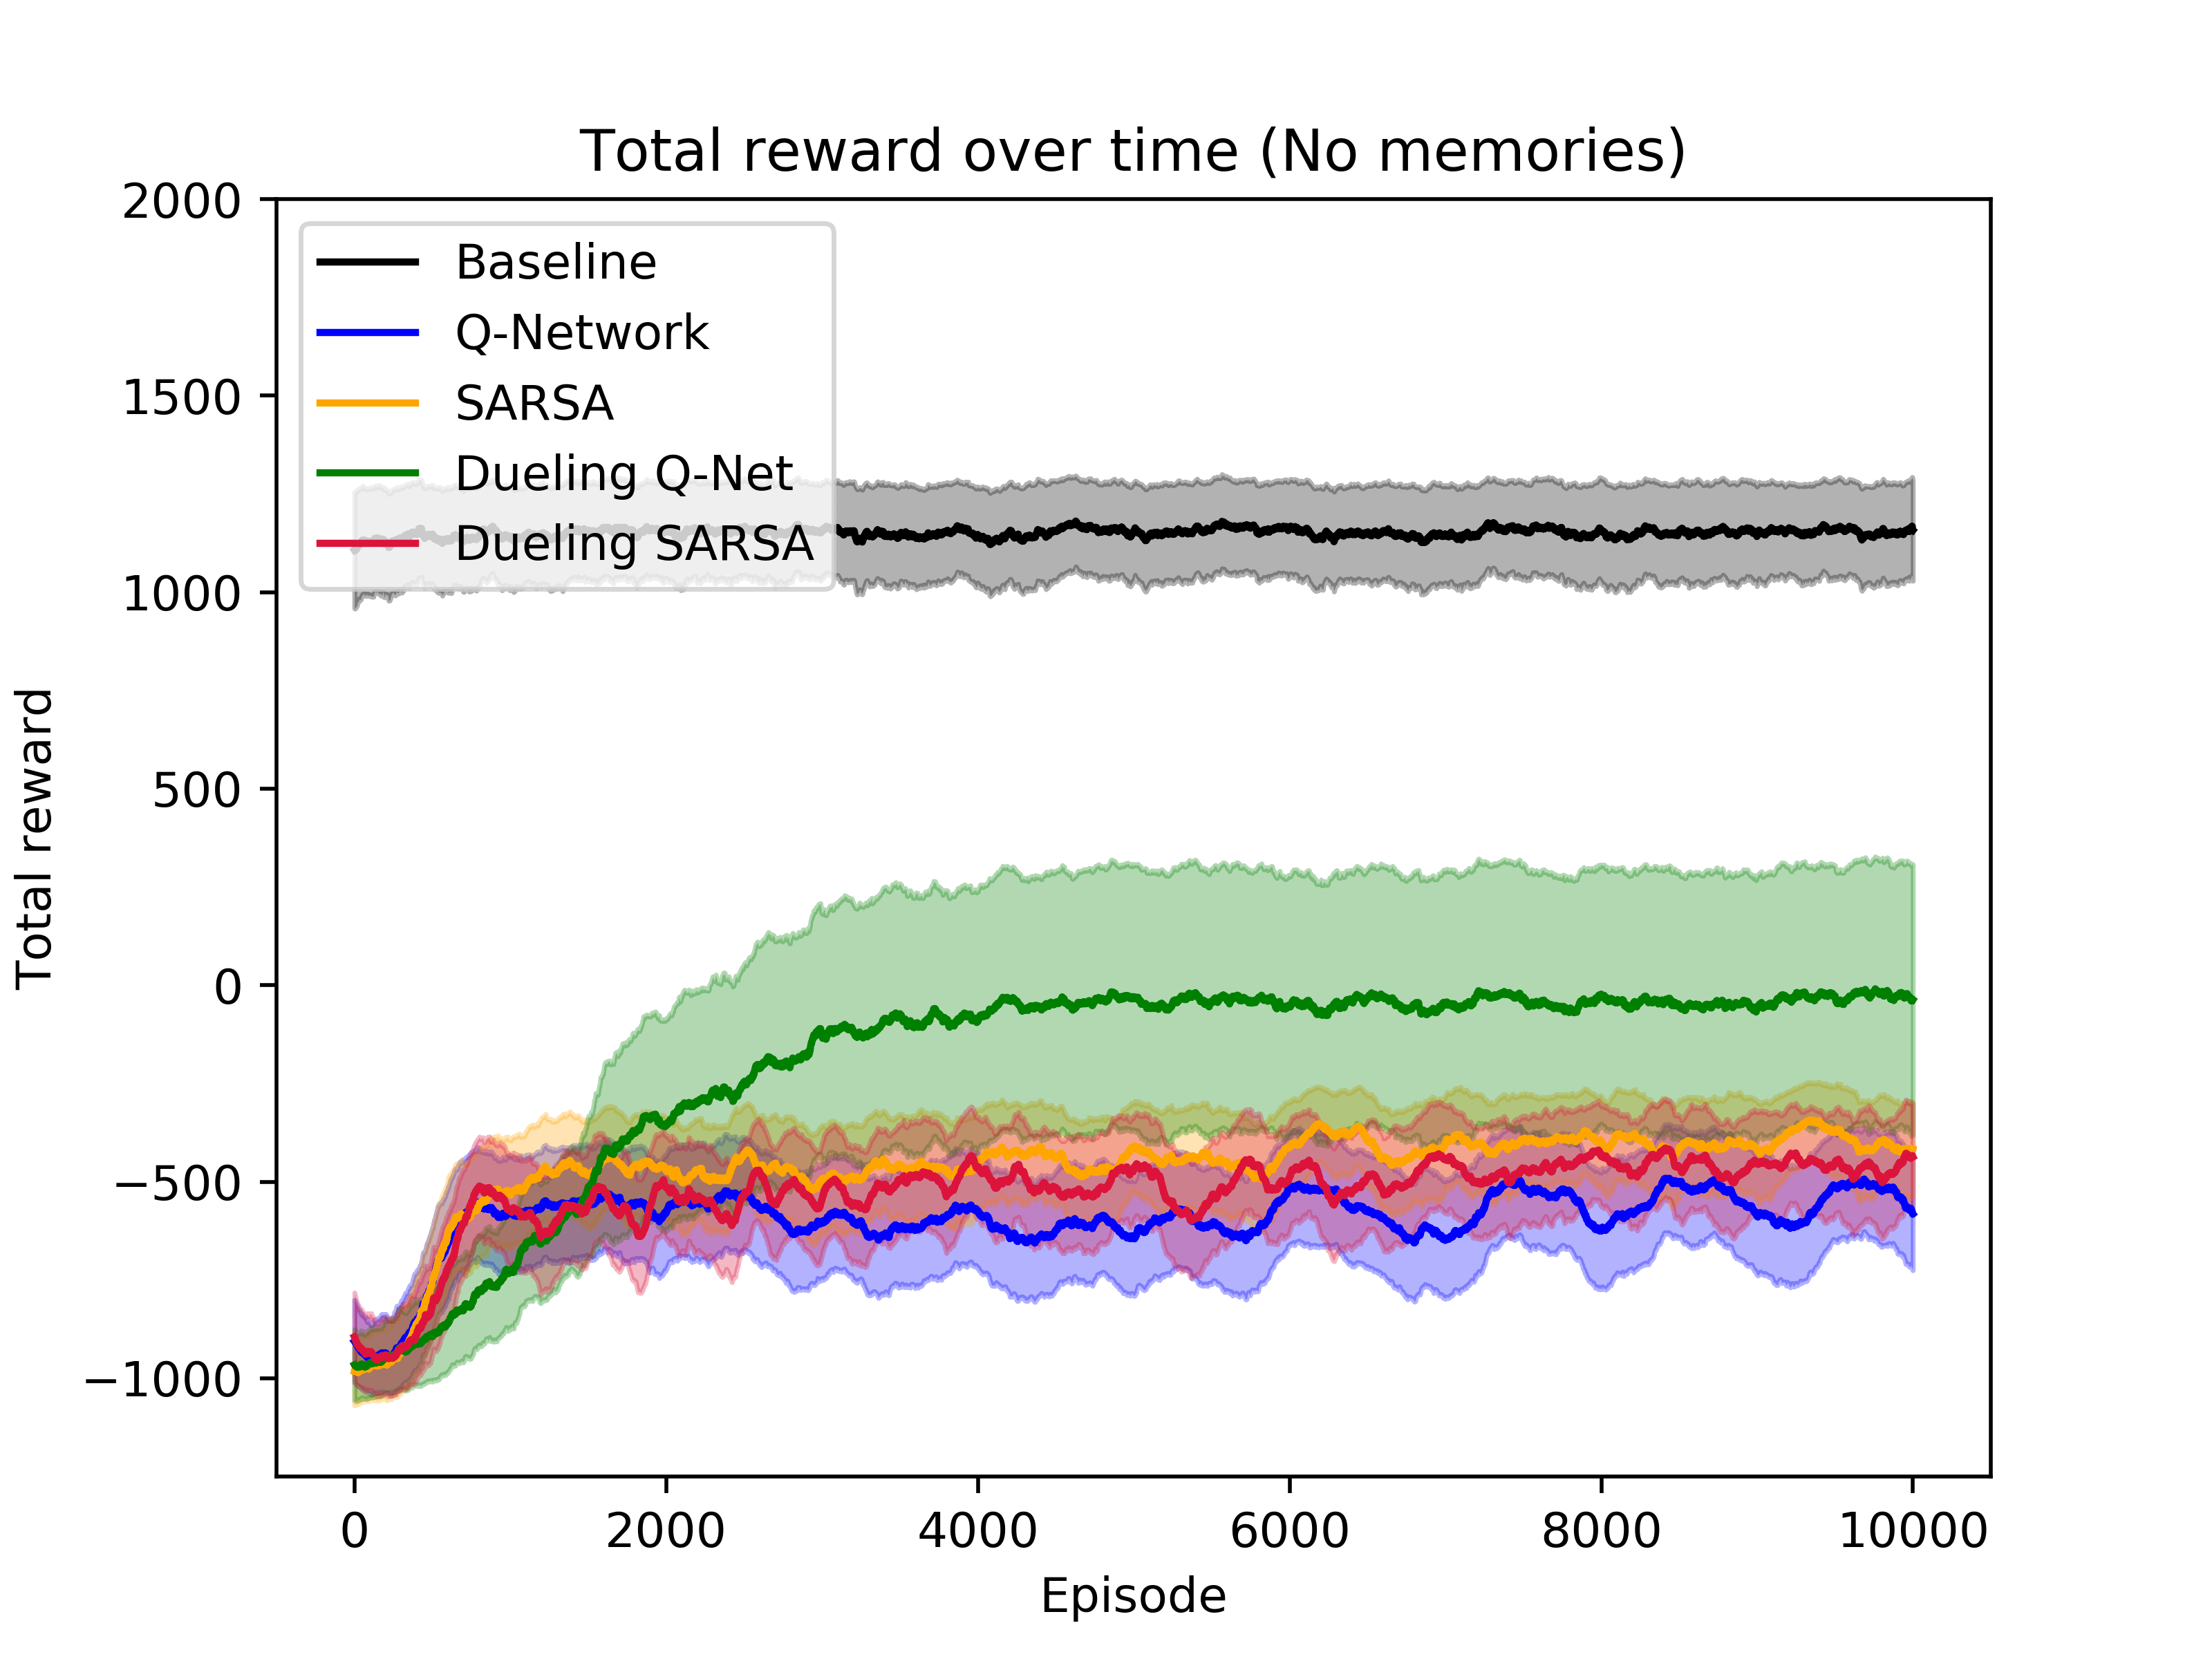
\includegraphics[width=\linewidth]{img/results/14-sized/total_rewards_0m-min.png}
    \caption{14-by-14 grid given no demonstation data.}
    \label{fig:14sized-nomem}
    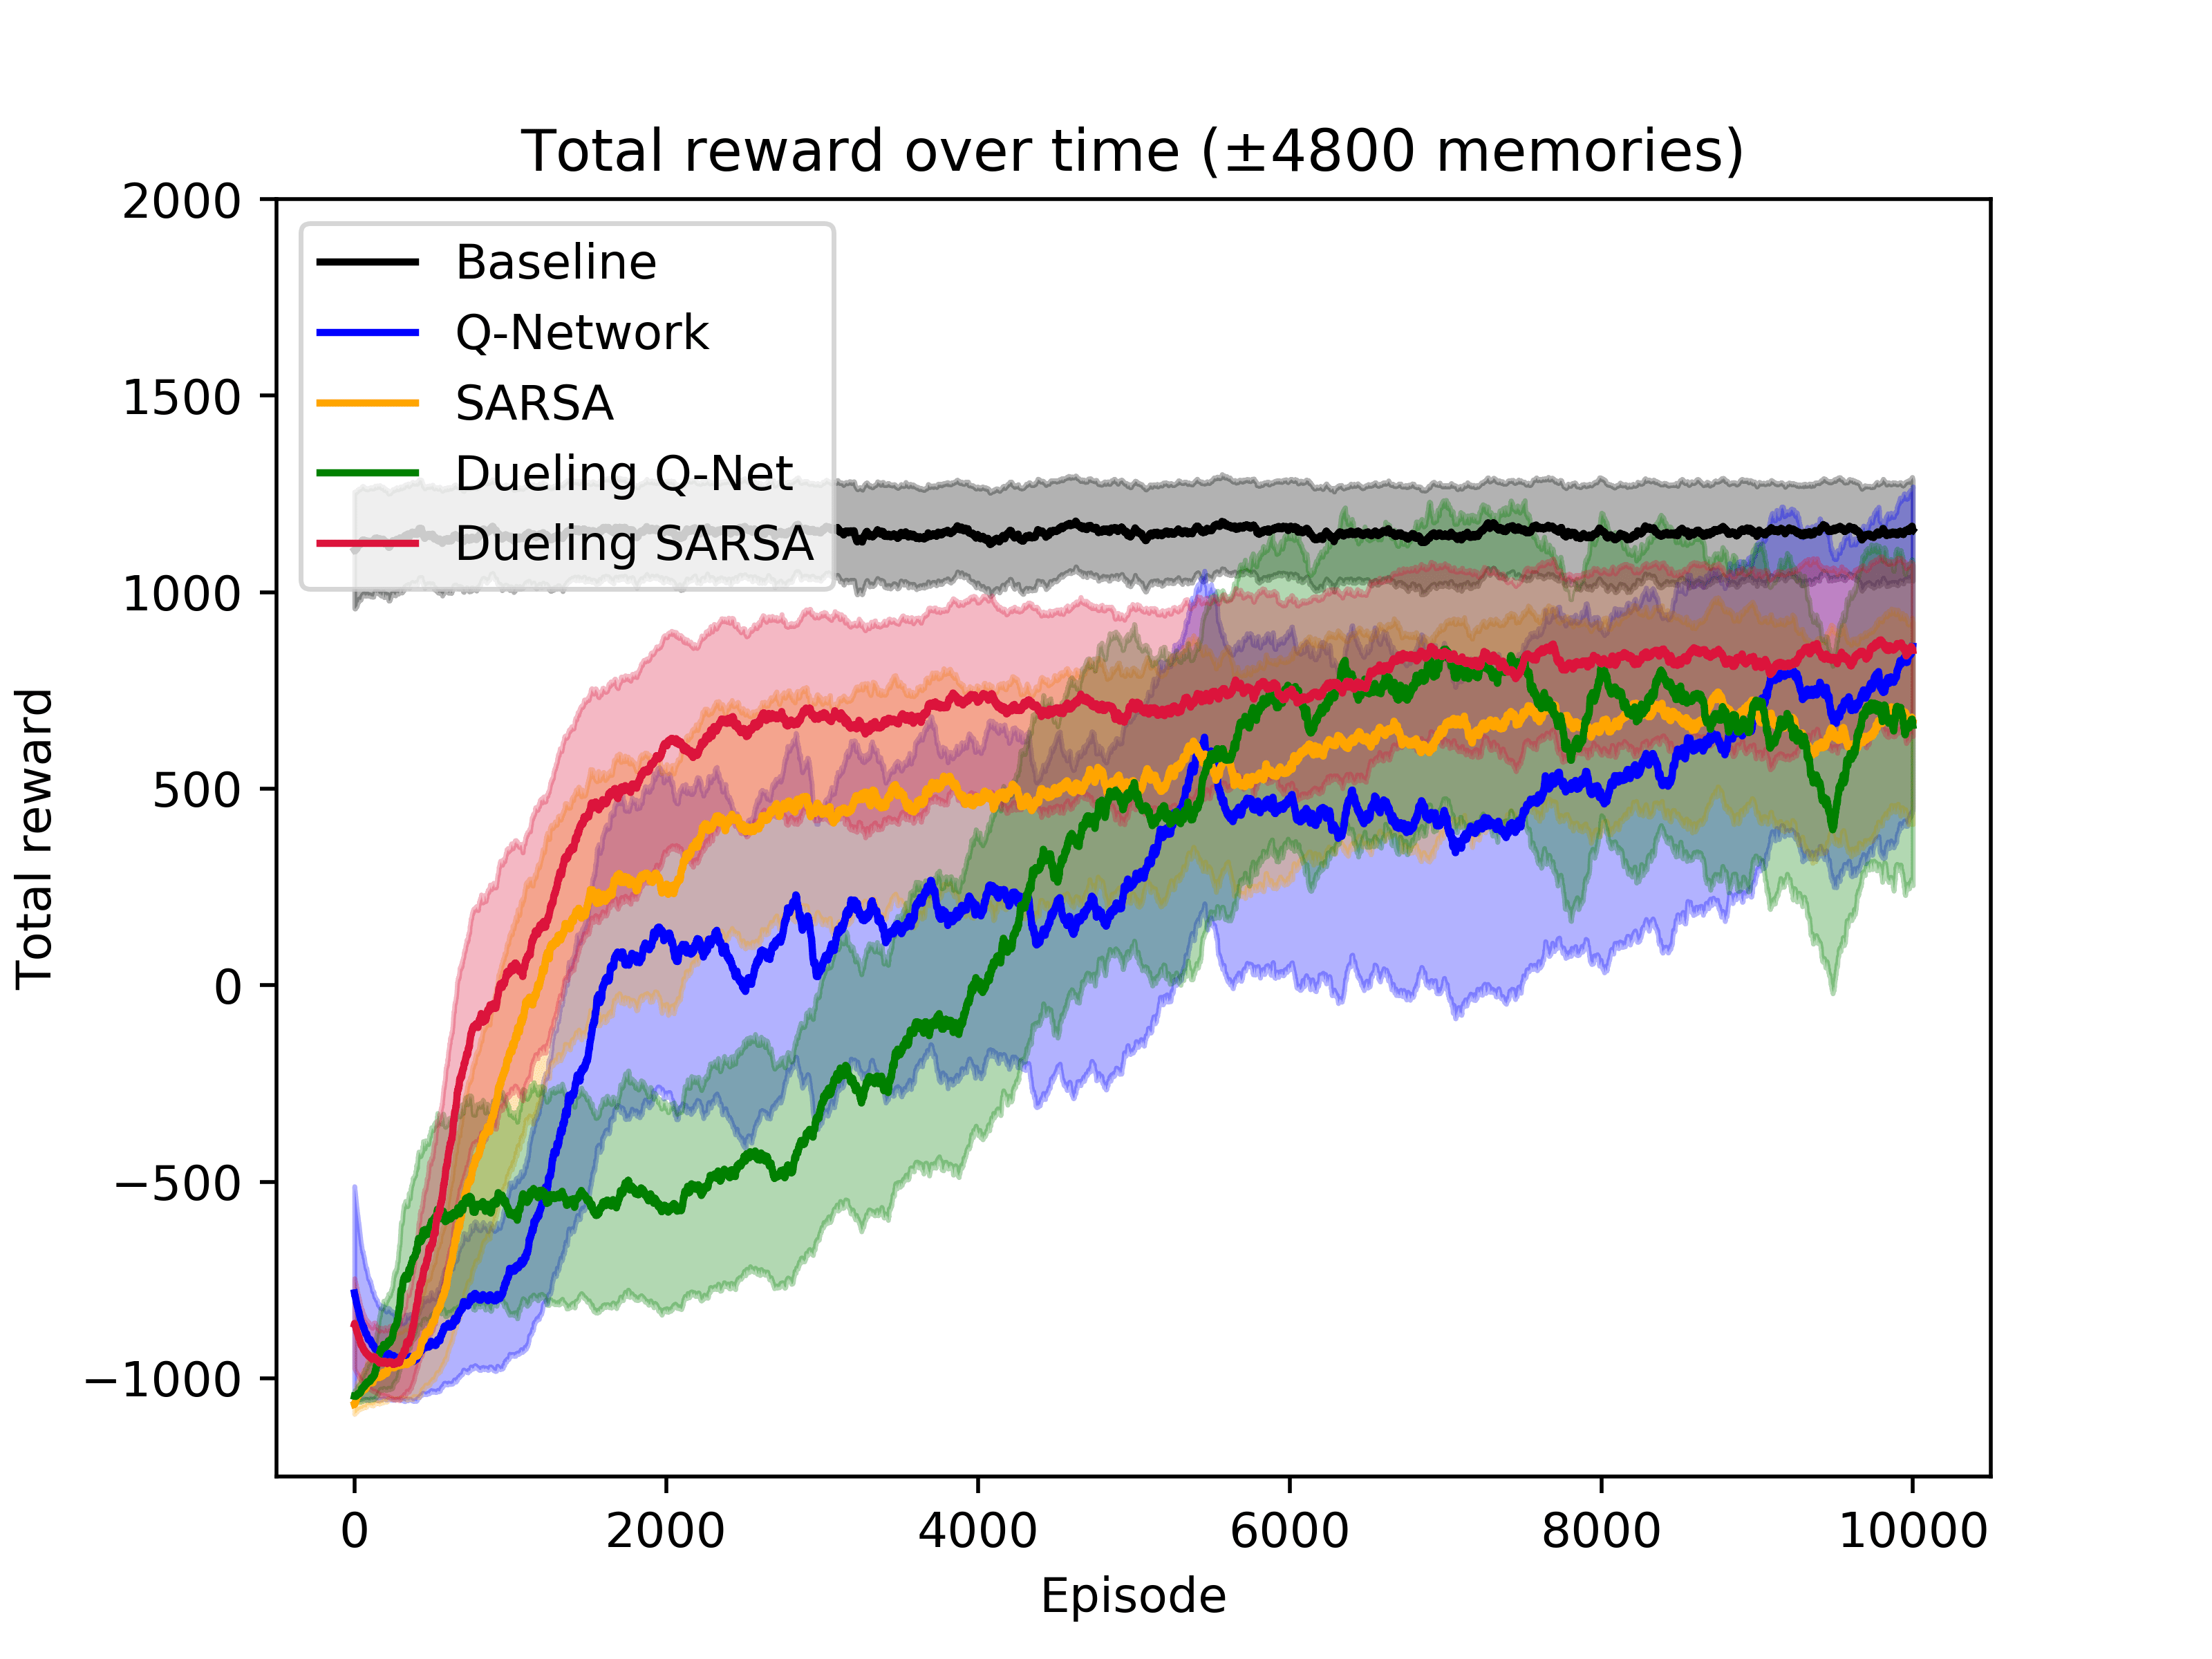
\includegraphics[width=\linewidth]{img/results/14-sized/total_rewards_100m-min.png}
    \caption{14-by-14 grid given 100 episodes of demonstation data.}
    \label{fig:14sized-100mem}
    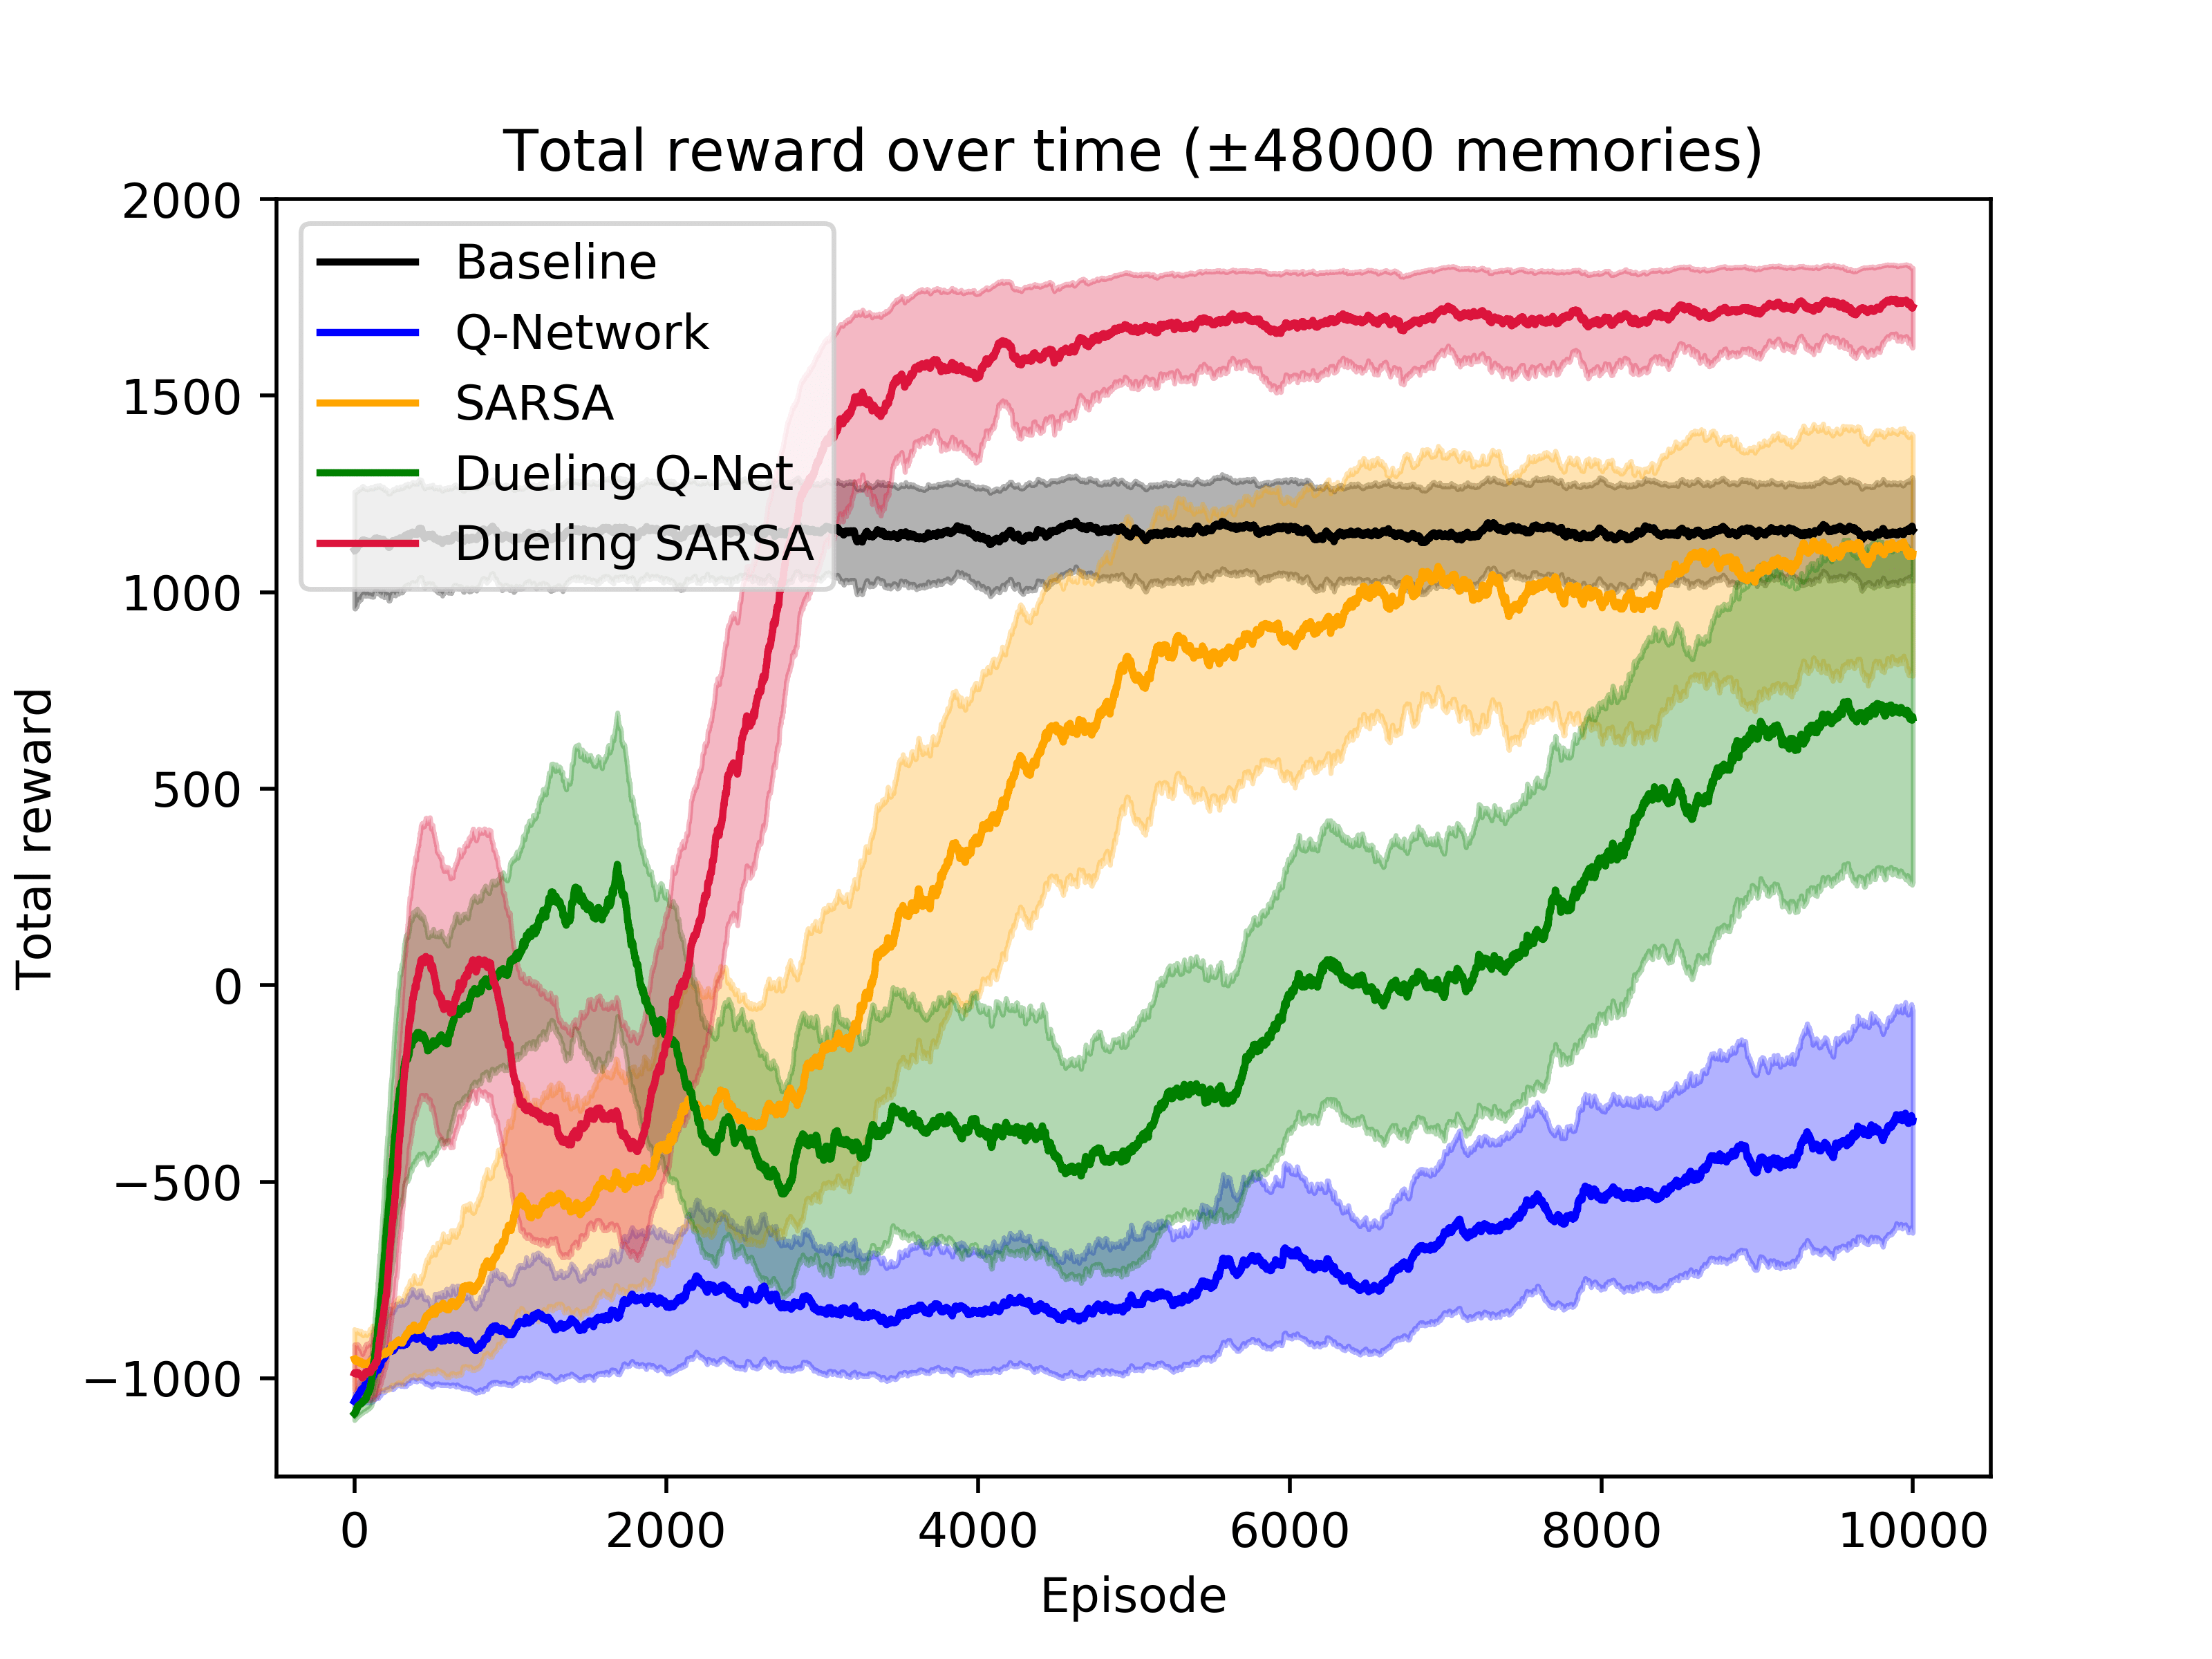
\includegraphics[width=\linewidth]{img/results/14-sized/total_rewards_1000m-min.png}
    \caption{14-by-14 grid given 1000 episodes of demonstation data.}
    \label{fig:14sized-1000mem}
\end{figure}


% SECOND-GEN TABLES
\begin{table}[H]
\begin{tabular}{l|l|l|l|}
\cline{2-4}
\textbf{} & Average Reward & Standard Error & Best Reward \\ \hline
\multicolumn{1}{|l|}{Size 10, no memories} & 1129 & 1.9 & 1387 \\ \hline
\multicolumn{1}{|l|}{Size 10, 100 memories} & 1129 & 1.9 & 1387 \\ \hline
\multicolumn{1}{|l|}{Size 10, 1000 memories} & 1129 & 1.9 & 1387 \\ \hline
\multicolumn{1}{|l|}{Size 14, no memories} & 1152 & 2.8 & 1513 \\ \hline
\multicolumn{1}{|l|}{Size 14, 100 memories} & 1152 & 2.8 & 1513 \\ \hline
\multicolumn{1}{|l|}{Size 14, 1000 memories} & 1152 & 2.8 & 1513 \\ \hline
\end{tabular}
\caption{Baseline rewards of the final 2500 episodes.}
\label{tab:2500base}
\end{table}
\begin{table}[H]
\begin{tabular}{l|l|l|l|}
\cline{2-4}
\textbf{} & Average Reward & Standard Error & Best Reward \\ \hline
\multicolumn{1}{|l|}{Size 10, no memories} & 221 & 4.2 & 715 \\ \hline
\multicolumn{1}{|l|}{Size 10, 100 memories} & 878 & 7.5 & \textbf{1758} \\ \hline
\multicolumn{1}{|l|}{Size 10, 1000 memories} & 907 & 6.7 & \textbf{1696} \\ \hline
\multicolumn{1}{|l|}{Size 14, no memories} & -550 & 2.9 & -139 \\ \hline
\multicolumn{1}{|l|}{Size 14, 100 memories} & 652 & 7.0 & \textbf{1629} \\ \hline
\multicolumn{1}{|l|}{Size 14, 1000 memories} & -459 & 5.0 & 411 \\ \hline
\end{tabular}
\caption{Q-Network rewards of the final 2500 episodes.}
\label{tab:2500qnet}
\end{table}
\begin{table}[H]
\begin{tabular}{l|l|l|l|}
\cline{2-4}
\textbf{} & Average Reward & Standard Error & Best Reward \\ \hline
\multicolumn{1}{|l|}{Size 10, no memories} & 956 & 4.1 & 1335 \\ \hline
\multicolumn{1}{|l|}{Size 10, 100 memories} & 521 & 6.8 & \textbf{1535} \\ \hline
\multicolumn{1}{|l|}{Size 10, 1000 memories} & \textbf{1369} & 5.5 & \textbf{1826} \\ \hline
\multicolumn{1}{|l|}{Size 14, no memories} & -40 & 3.0 & 349 \\ \hline
\multicolumn{1}{|l|}{Size 14, 100 memories} & 667 & 7.8 & \textbf{1748} \\ \hline
\multicolumn{1}{|l|}{Size 14, 1000 memories} & 522 & 7.7 & \textbf{1534} \\ \hline
\end{tabular}
\caption{Dueling Q-Network rewards of the final 2500 episodes.}
\label{tab:2500duel}
\end{table}
\begin{table}[H]
\begin{tabular}{l|l|l|l|}
\cline{2-4}
\textbf{} & Average Reward & Standard Error & Best Reward \\ \hline
\multicolumn{1}{|l|}{Size 10, no memories} & 132 & 3.9 & 563 \\ \hline
\multicolumn{1}{|l|}{Size 10, 100 memories} & 776 & 4.7 & 1292 \\ \hline
\multicolumn{1}{|l|}{Size 10, 1000 memories} & \textbf{1607} & 2.8 & \textbf{1748} \\ \hline
\multicolumn{1}{|l|}{Size 14, no memories} & -398 & 2.4 & -92 \\ \hline
\multicolumn{1}{|l|}{Size 14, 100 memories} & 670 & 5.3 & 1275 \\ \hline
\multicolumn{1}{|l|}{Size 14, 1000 memories} & 1057 & 5.6 & \textbf{1626} \\ \hline
\end{tabular}
\caption{SARSA rewards of the final 2500 episodes.}
\label{tab:2500sarsa}
\end{table}
\clearpage
\begin{table}[H]
\begin{tabular}{l|l|l|l|}
\cline{2-4}
\textbf{} & Average Reward & Standard Error & Best Reward \\ \hline
\multicolumn{1}{|l|}{Size 10, no memories} & 241 & 2.6 & 582 \\ \hline
\multicolumn{1}{|l|}{Size 10, 100 memories} & 1031 & 3.4 & 1312 \\ \hline
\multicolumn{1}{|l|}{Size 10, 1000 memories} & \textbf{1745} & 2.5 & \textbf{1860} \\ \hline
\multicolumn{1}{|l|}{Size 14, no memories} & -455 & 2.6 & -44 \\ \hline
\multicolumn{1}{|l|}{Size 14, 100 memories} & 836 & 4.1 & 1249 \\ \hline
\multicolumn{1}{|l|}{Size 14, 1000 memories} & \textbf{1713} & 3.0 & \textbf{1846} \\ \hline
\end{tabular}
\caption{Dueling SARSA rewards of the final 2500 episodes.}
\label{tab:2500duel}
\end{table}


% HYPERPARAMETERS
\begin{table}[H]
\begin{tabular}{|l|l|}
\hline
Memory size & 20000 \\ \hline
Batch size & 32 \\ \hline
Target update (C) & 20 \\ \hline
Gamma (X) & 0.999 \\ \hline
Alpha (X) & 0.005 \\ \hline
Epsilon decay (X) & 0.01 \\ \hline
Epsilon minimum & 1 \\ \hline
Epsilon maximum & 0.005 \\ \hline
\end{tabular}
\caption{All relevant hyper-parameters used in the training process.}
\label{tab:hyperparameters}
\end{table}


\clearpage
\section*{Probably exclude these..}
% FIRST-GEN TABLES
\begin{table}[H]
\begin{tabular}{|l|r|r|r|r|r|}
\hline
\textbf{Experiment Setup} & \multicolumn{1}{l|}{\textbf{Baseline}} & \multicolumn{1}{l|}{\textbf{Q-Network}} & \multicolumn{1}{l|}{\textbf{SARSA}} & \multicolumn{1}{l|}{\textbf{\begin{tabular}[c]{@{}l@{}}Dueling\\ Q-Network\end{tabular}}} & \multicolumn{1}{l|}{\textbf{\begin{tabular}[c]{@{}l@{}}Dueling\\ SARSA\end{tabular}}} \\ \hline
Size 10, no memories & 1130.2 & -81.5 & -149.6 & 692.1 & -9.4 \\ \hline
Size 10, 100 memories & 1130.2 & 869.0 & 642.5 & 470.7 & 845.4 \\ \hline
Size 10, 1000 memories & 1130.2 & 98.9 & 1017.5 & 825.6 & \textbf{1333.9} \\ \hline
Size 14, no memories & 1151.4 & -590.5 & -460.9 & -188.8 & -523.2 \\ \hline
Size 14, 100 memories & 1151.4 & -220.5 & 412.6 & 197.4 & 604.5 \\ \hline
Size 14, 1000 memories & 1151.4 & -708.8 & 421.8 & -11.8 & \textbf{1194.0} \\ \hline
\end{tabular}
\caption{Averaged rewards from all training episodes.}
\label{tab:averages}
\end{table}
\begin{table}[H]
\begin{tabular}{|l|r|r|r|r|r|}
\hline
\textbf{Experiment Setup} & \multicolumn{1}{l|}{\textbf{Baseline}} & \multicolumn{1}{l|}{\textbf{Q-Network}} & \multicolumn{1}{l|}{\textbf{SARSA}} & \multicolumn{1}{l|}{\textbf{\begin{tabular}[c]{@{}l@{}}Dueling\\ Q-Network\end{tabular}}} & \multicolumn{1}{l|}{\textbf{\begin{tabular}[c]{@{}l@{}}Dueling\\ SARSA\end{tabular}}} \\ \hline
Size 10, no memories & 1265.8 & 435.7 & 327.0 & 1187.8 & 382.0 \\ \hline
Size 10, 100 memories & 1265.8 & \textbf{1608.8} & 1159.1 & \textbf{1272.0} & 1255.1 \\ \hline
Size 10, 1000 memories & 1265.8 & 1243.7 & \textbf{1726.6} & \textbf{1730.8} & \textbf{1832.6} \\ \hline
Size 14, no memories & 1363.4 & -326.3 & -226.2 & 177.5 & -262.7 \\ \hline
Size 14, 100 memories & 1363.4 & 1049.0 & 1028.0 & 1225.5 & 1112.0 \\ \hline
Size 14, 1000 memories & 1363.4 & -181.3 & \textbf{1393.9} & 912.5 & \textbf{1830.2} \\ \hline
\end{tabular}
\caption{Averaged rewards from the best 1000 training episodes.}
\label{tab:best10averages}
\end{table}
\begin{table}[H]
\begin{tabular}{|l|r|r|r|r|r|}
\hline
\textbf{Experiment Setup} & \multicolumn{1}{l|}{\textbf{Baseline}} & \multicolumn{1}{l|}{\textbf{Q-Network}} & \multicolumn{1}{l|}{\textbf{SARSA}} & \multicolumn{1}{l|}{\textbf{\begin{tabular}[c]{@{}l@{}}Dueling\\ Q-Network\end{tabular}}} & \multicolumn{1}{l|}{\textbf{\begin{tabular}[c]{@{}l@{}}Dueling\\ SARSA\end{tabular}}} \\ \hline
Size 10, no memories & 1132.3 & 253.6 & 180.5 & 973.4 & 255.0 \\ \hline
Size 10, 100 memories & 1132.3 & 692.5 & 791.5 & 548.3 & 1040.7 \\ \hline
Size 10, 1000 memories & 1132.3 & 977.2 & \textbf{1591.9} & \textbf{1297.5} & \textbf{1751.3} \\ \hline
Size 14, no memories & 1155.4 & -551.0 & -391.5 & -28.1 & -457.0 \\ \hline
Size 14, 100 memories & 1155.4 & 772.7 & 647.1 & 614.0 & 841.6 \\ \hline
Size 14, 1000 memories & 1155.4 & -387.3 & 1102.7 & 674.4 & \textbf{1729.1} \\ \hline
\end{tabular}
\caption{Averaged rewards from the final 1000 training episodes.}
\label{tab:last10averages}
\end{table}